\chapter{Feature selection and important: Biomedical analysis}


\section{Data}

The dataset contains anonymized biomedical data and is composed of a binary target variable and unknown variables.

\begin{remark}
    In reality, this dataset contains real-world examples. Features have been anonymized for the purpose of feature analysis.
\end{remark}


\subsection{Preliminary analysis}

\begin{description}
    \item[Data distribution]
        There are both categorical and numerical features.
        \begin{figure}[H]
            \centering
            \begin{subfigure}{0.75\linewidth}
                \centering
                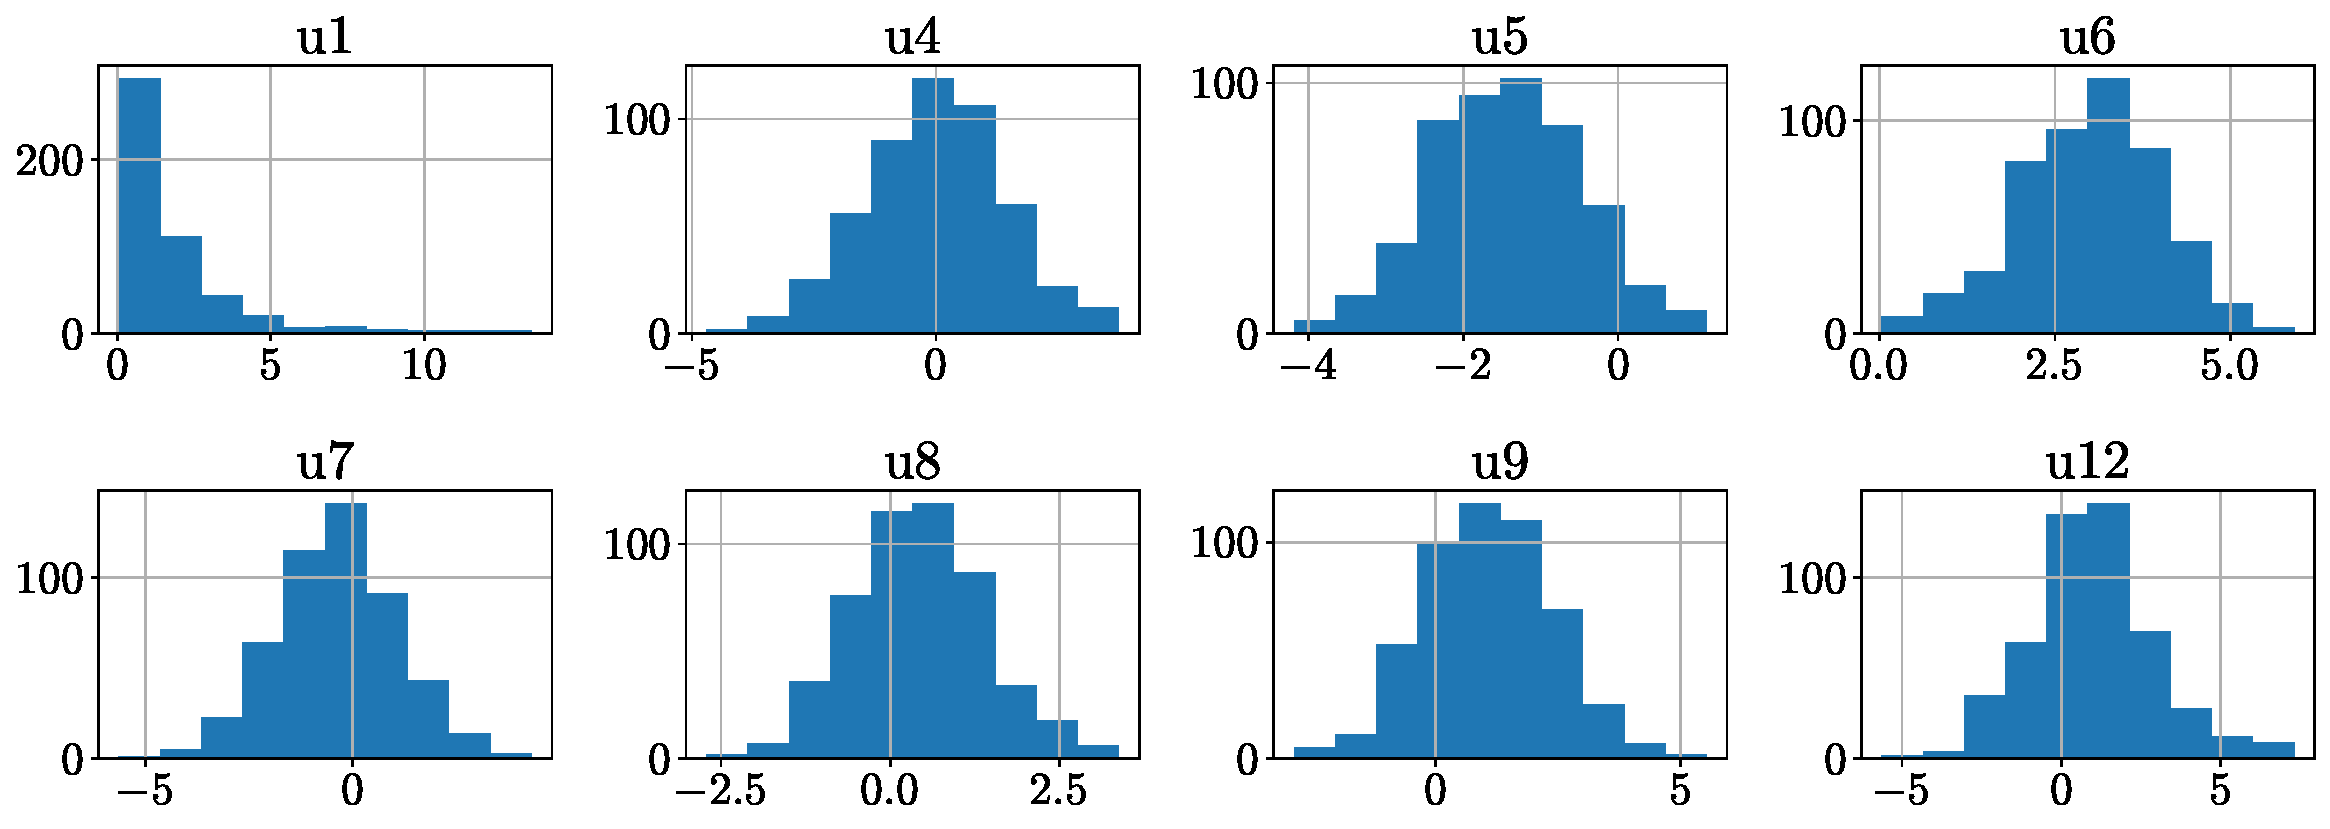
\includegraphics[width=\linewidth]{./img/_biomed_numeric_distr.pdf}
                \caption{Numerical features}
            \end{subfigure}
            \begin{subfigure}{0.75\linewidth}
                \centering
                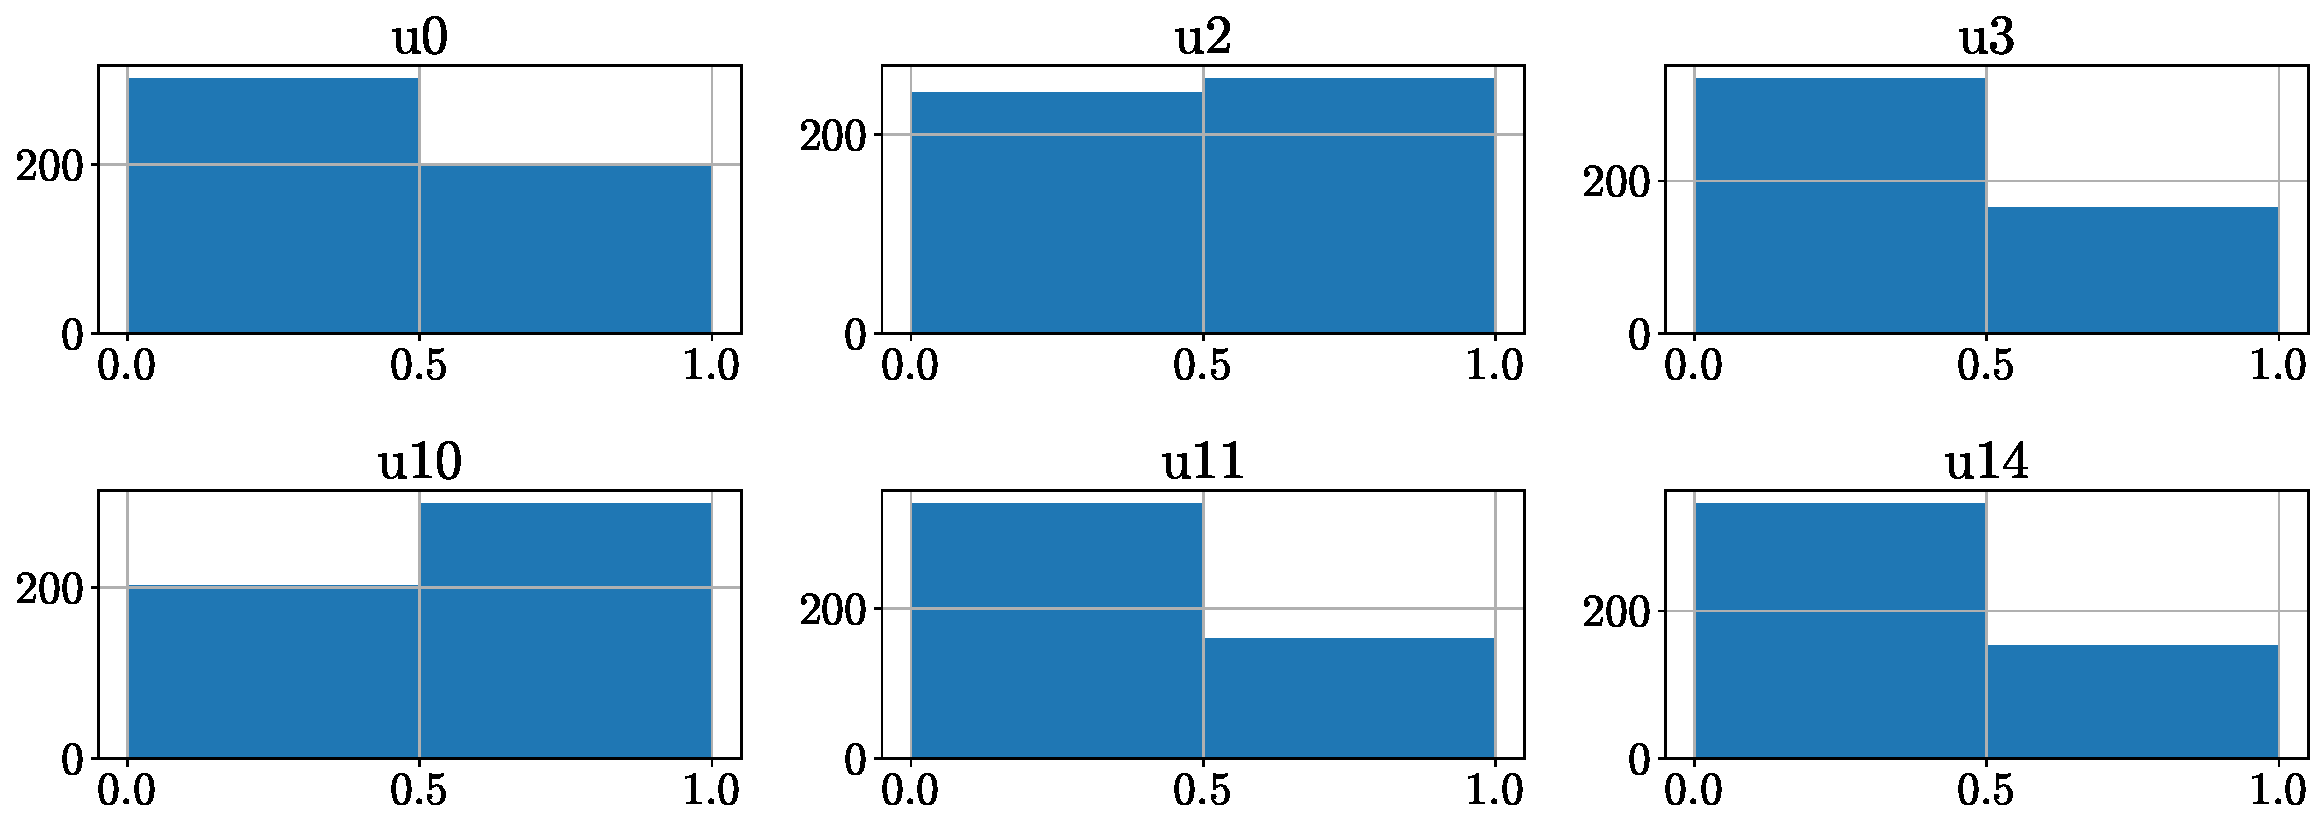
\includegraphics[width=\linewidth]{./img/_biomed_categ_distr.pdf}
                \caption{Categorical features}
            \end{subfigure}
            \begin{subfigure}{0.2\linewidth}
                \centering
                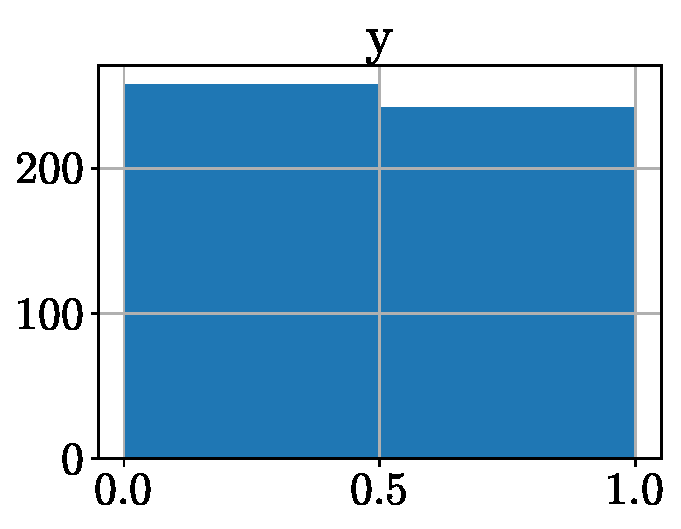
\includegraphics[width=\linewidth]{./img/_biomed_target_distr.pdf}
                \caption{Target}
            \end{subfigure}
            \caption{Distribution of the dataset}
        \end{figure}

    \item[Univariate dependencies]
        Determine the fraction of examples with target $Y=1$ (i.e., likelihood that a feature has a specific value while the target is $1$).

        \begin{figure}[H]
            \centering
            \begin{subfigure}{0.75\linewidth}
                \centering
                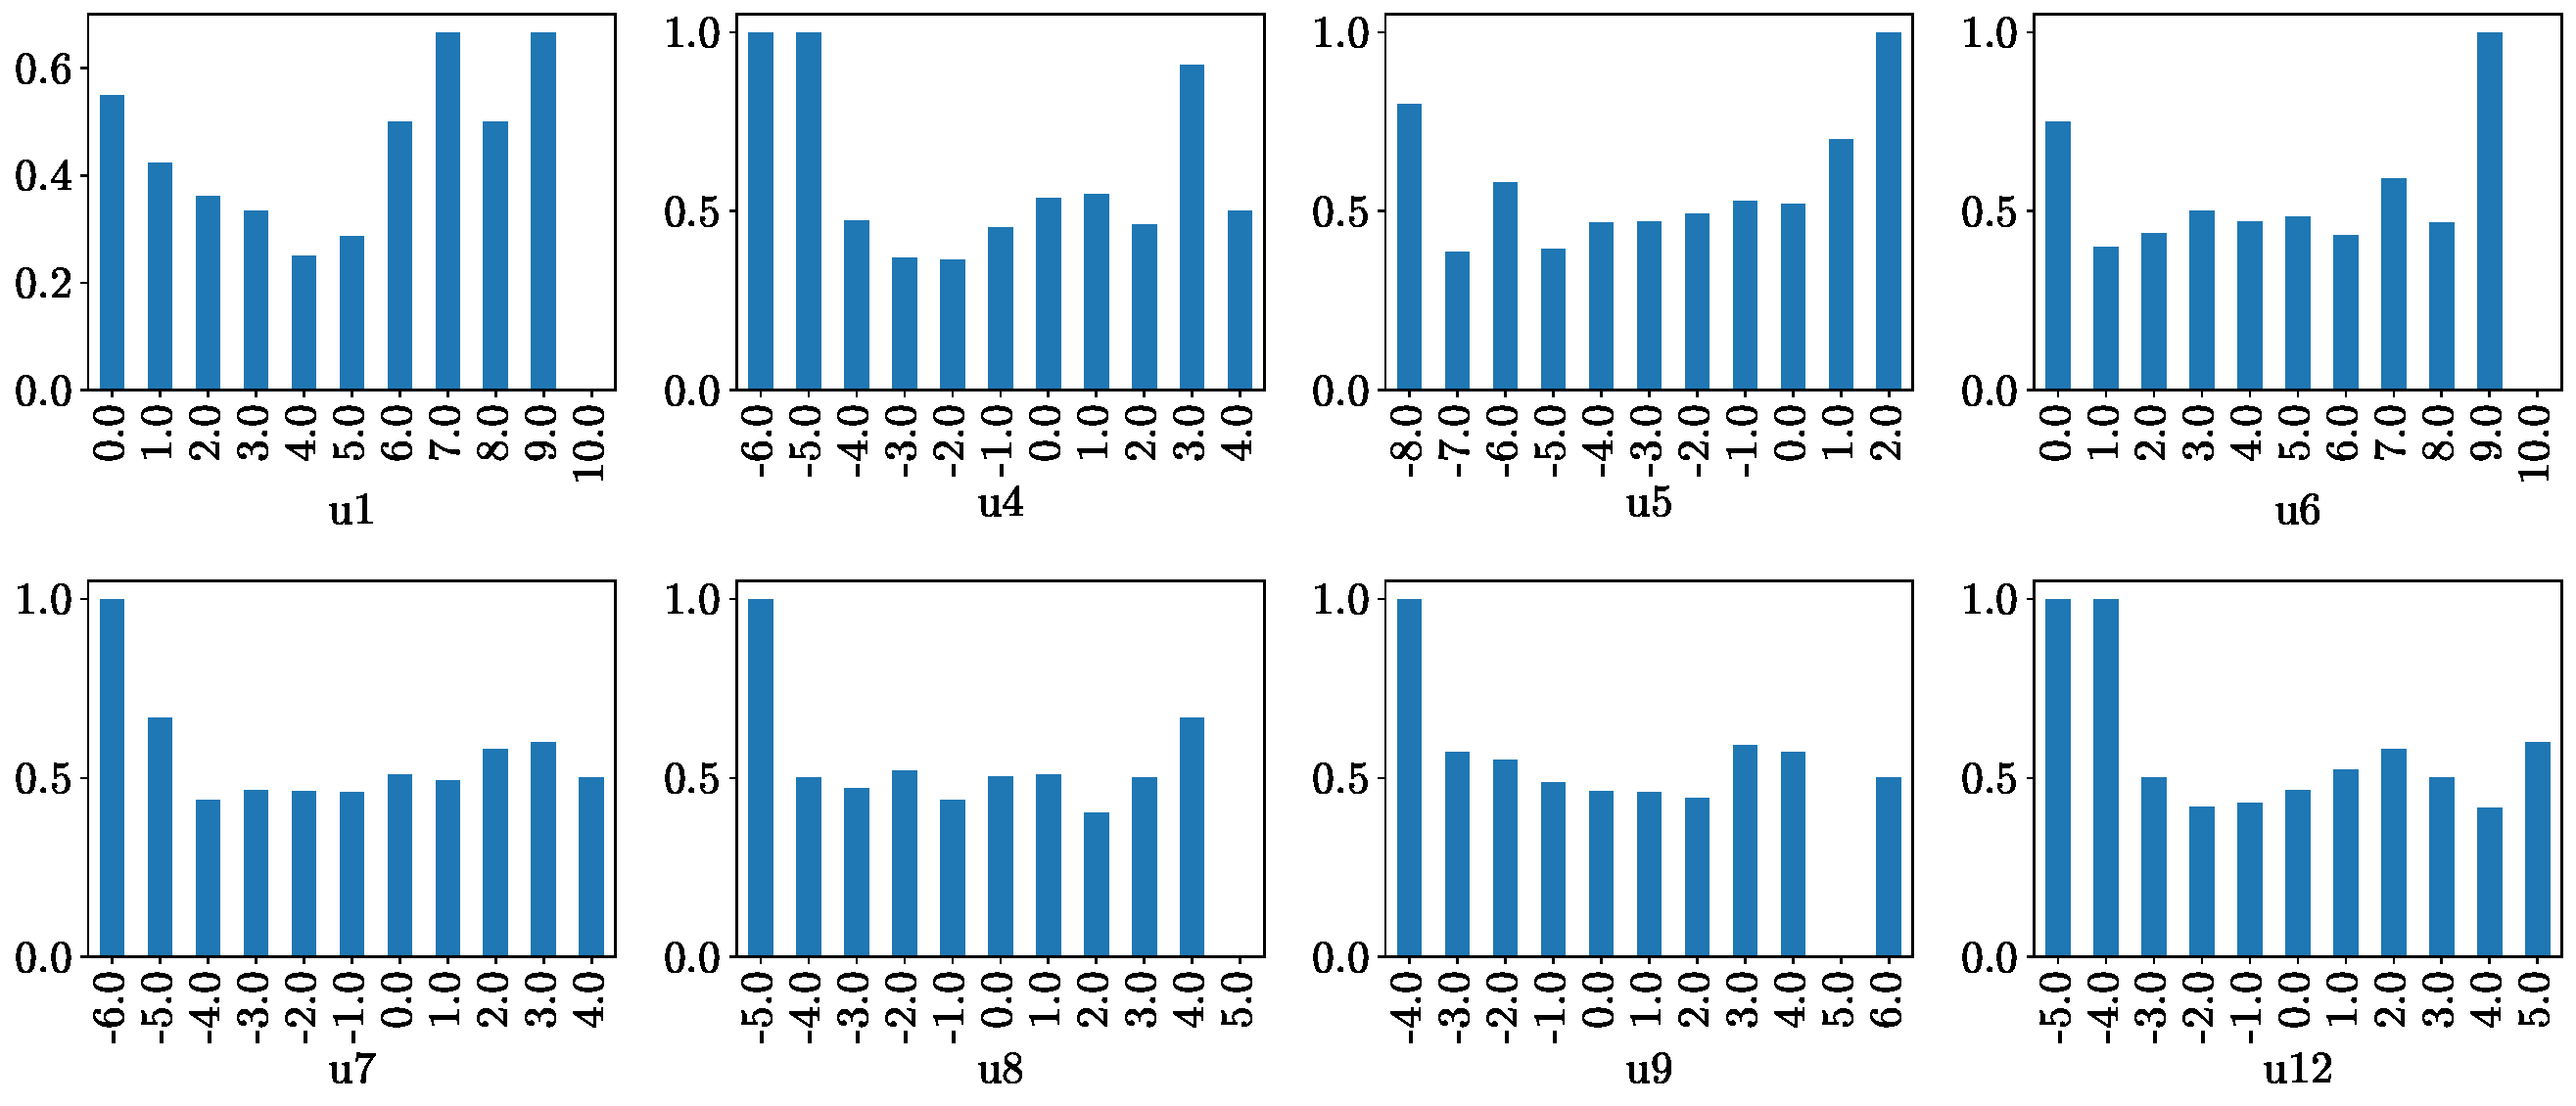
\includegraphics[width=\linewidth]{./img/_biomed_target_num_distr.pdf}
                \caption{Numerical features}
            \end{subfigure}
            \begin{subfigure}{0.75\linewidth}
                \centering
                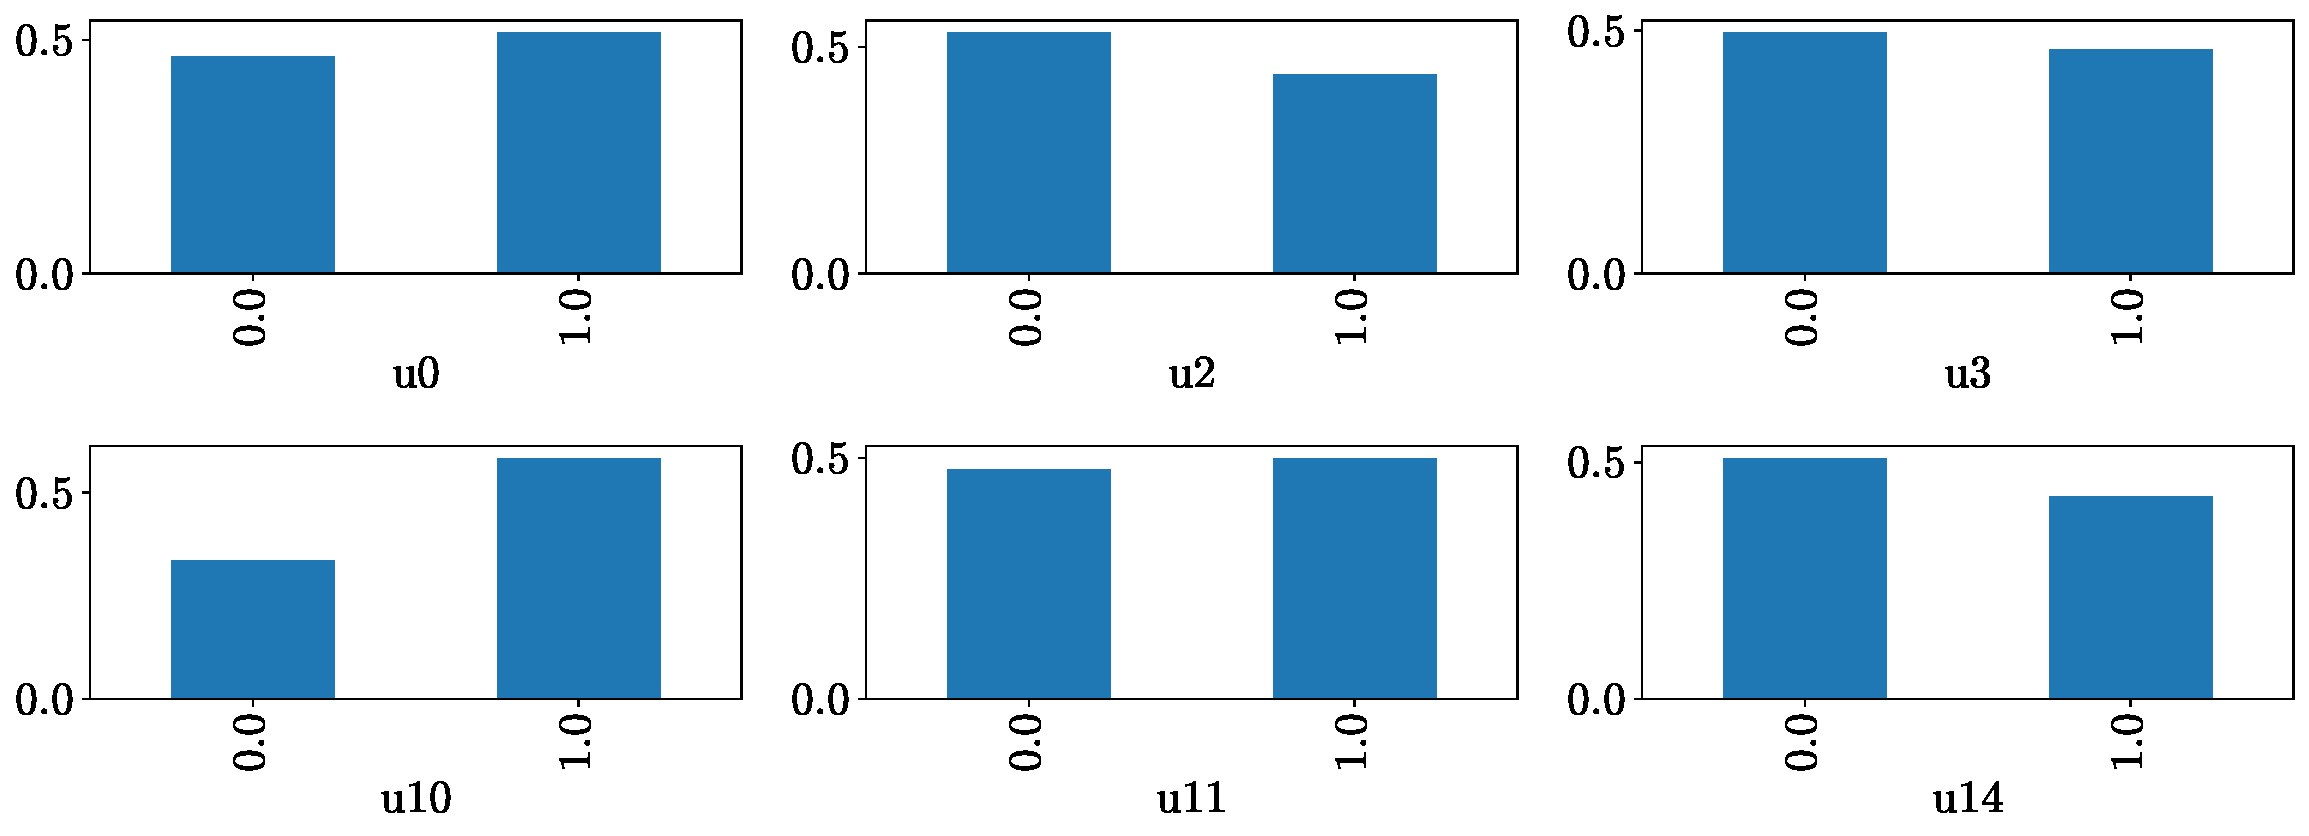
\includegraphics[width=\linewidth]{./img/_biomed_target_categ_distr.pdf}
                \caption{Categorical features}
            \end{subfigure}
            \caption{Univariate dependencies with $Y=1$}
        \end{figure}

    \item[Linear correlation]
        Determine the Pearson's correlation between variables.
        
        \begin{figure}[H]
            \centering
            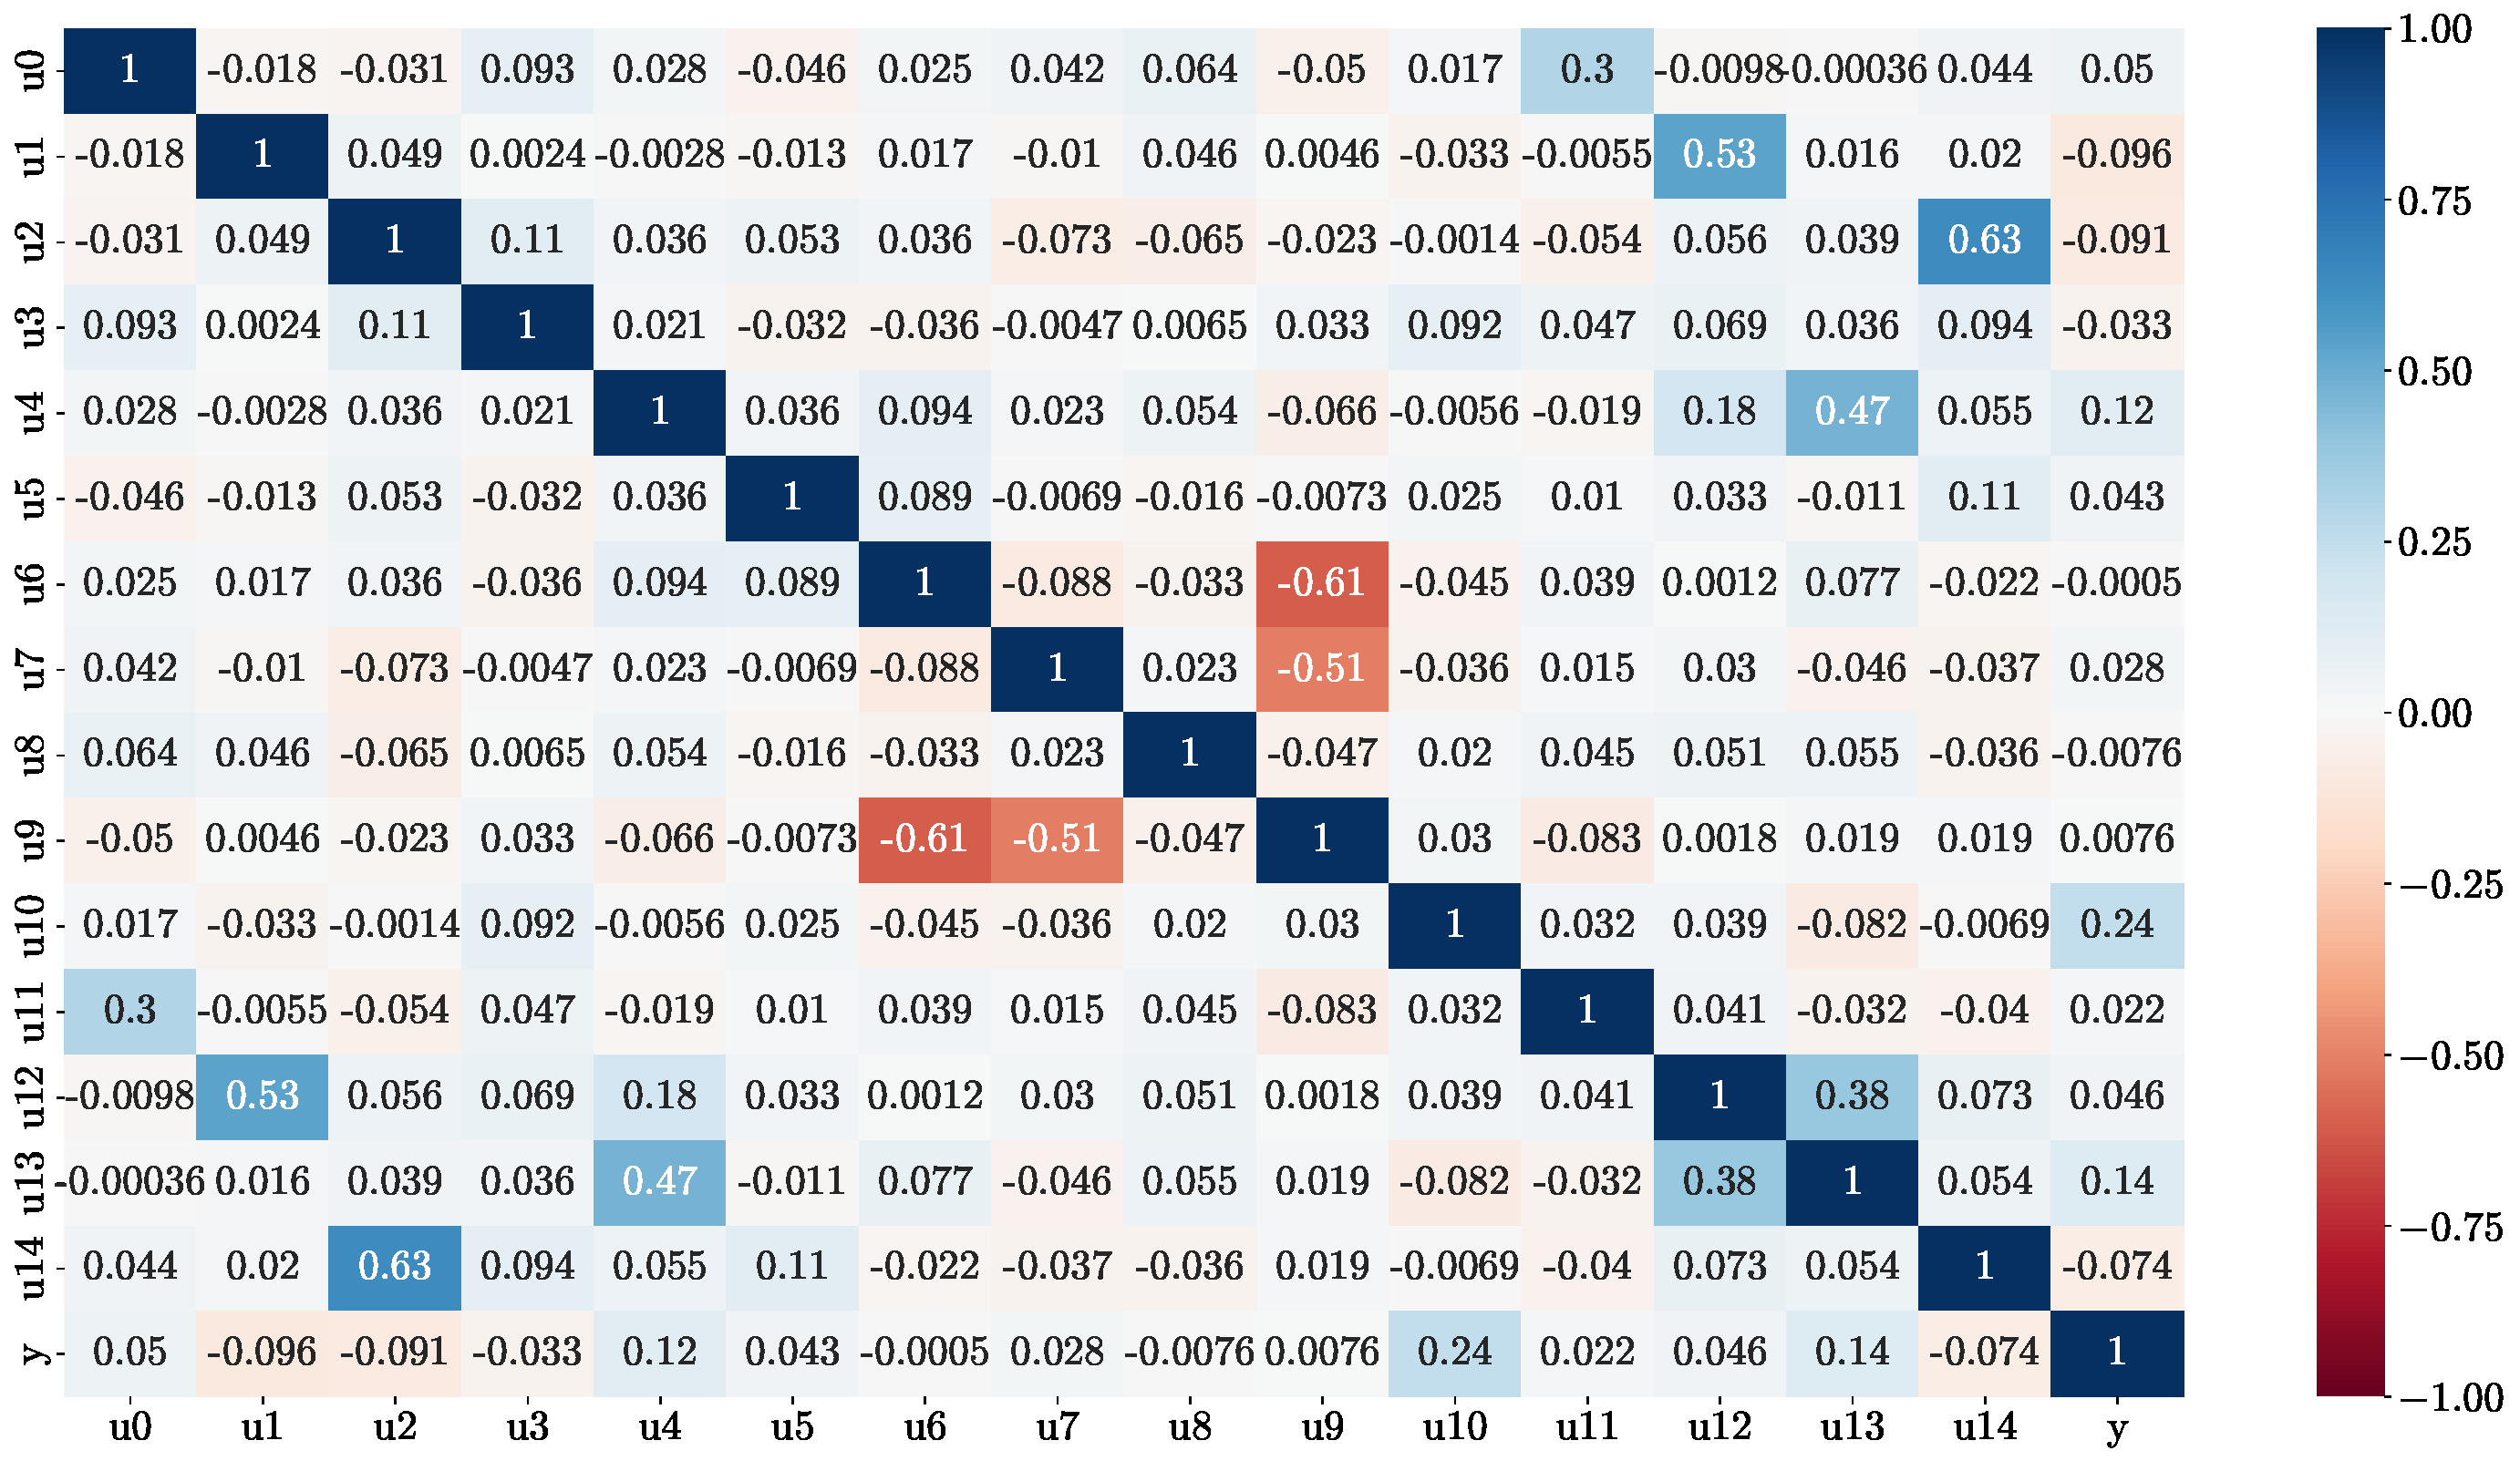
\includegraphics[width=0.8\linewidth]{./img/_biomed_corr_matrix.pdf}
        \end{figure}
\end{description}